\documentclass[border=10pt]{standalone}
\usepackage{amsmath}
\usepackage{tikz}
\usetikzlibrary{positioning, arrows.meta, calc, fit, backgrounds, shapes.geometric}
\begin{document}
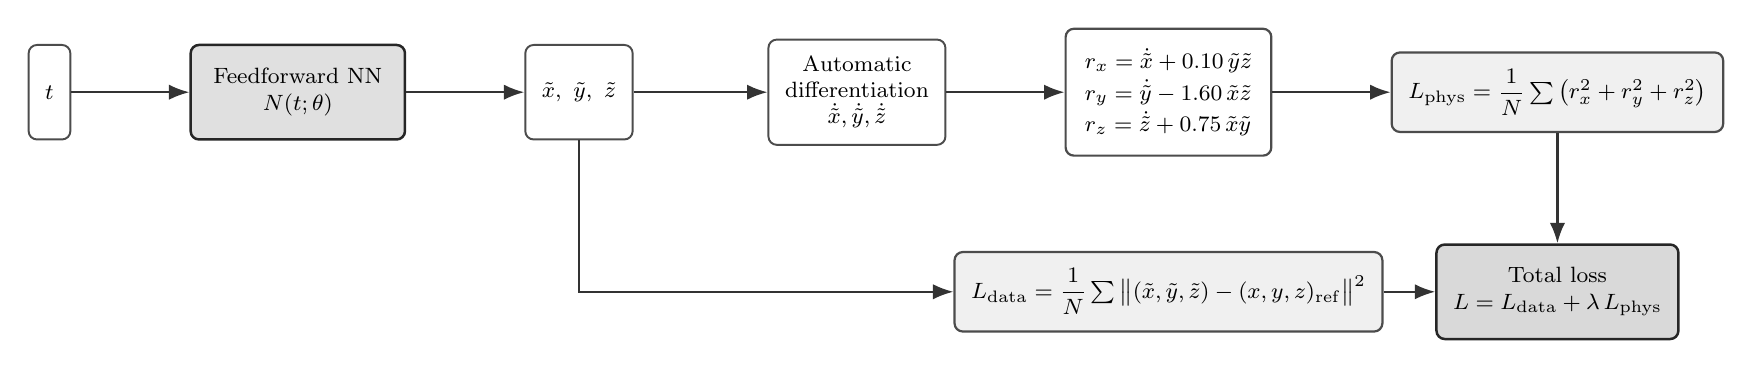
\begin{tikzpicture}[
    font=\footnotesize, node distance=1.0cm and 1.5cm,
    block/.style={rounded corners=3pt, draw=black!70, fill=white, line width=0.7pt,
                  align=center, inner sep=6pt, minimum height=1.2cm},
    nn/.style={rounded corners=3pt, draw=black!85, fill=black!12, line width=0.9pt,
               align=center, inner sep=6pt, minimum height=1.2cm, text width=2.3cm},
    res/.style={rounded corners=3pt, draw=black!70, fill=white, line width=0.8pt,
                align=left, inner sep=7pt},
    loss/.style={rounded corners=3pt, draw=black!70, fill=black!6, line width=0.8pt,
                 align=center, inner sep=6pt, minimum height=1.0cm},
    flow/.style={-{Latex[length=2.6mm]}, line width=0.8pt, draw=black!80}
]
\node[block] (t) {$t$};
\node[nn, right=of t] (net) {Feedforward NN\\$N(t;\theta)$};
\node[block, right=of net] (out) {$\tilde{x},\ \tilde{y},\ \tilde{z}$};
\node[block, right=1.7cm of out] (ad) {Automatic\\differentiation\\$\dot{\tilde{x}},\dot{\tilde{y}},\dot{\tilde{z}}$};
\node[res, right=of ad] (residual) {%
  $r_x=\dot{\tilde{x}}+0.10\,\tilde{y}\tilde{z}$\\[2pt]
  $r_y=\dot{\tilde{y}}-1.60\,\tilde{x}\tilde{z}$\\[2pt]
  $r_z=\dot{\tilde{z}}+0.75\,\tilde{x}\tilde{y}$};
\node[loss, right=of residual] (lphys) {$L_{\mathrm{phys}}=\dfrac{1}{N}\sum\big(r_x^2+r_y^2+r_z^2\big)$};
\node[block, below=1.4cm of lphys, fill=black!15, draw=black!85, line width=0.9pt] (total)
     {Total loss\\$L=L_{\mathrm{data}}+\lambda\,L_{\mathrm{phys}}$};
\node[loss] (ldata) at (residual |- total)
     {$L_{\mathrm{data}}=\dfrac{1}{N}\sum\big\|(\tilde{x},\tilde{y},\tilde{z})-(x,y,z)_{\mathrm{ref}}\big\|^2$};
\foreach \a/\b in {t/net, net/out, out/ad, ad/residual, residual/lphys}{\draw[flow] (\a)--(\b);}
\draw[flow] (out.south) |- (ldata.west);
\draw[flow] (lphys) -- (total);
\draw[flow] (ldata) -- (total);
\end{tikzpicture}
\end{document}
